\documentclass[conference]{IEEEtran}

\usepackage{cite}
\usepackage{graphicx}
\usepackage{url}

\title{From DRS to Mario Mushrooms: Visualizing Early-Season Formula 1 Change Across 2025 and 2026}

\author{\IEEEauthorblockN{Alejandro Gonzalez}
\IEEEauthorblockA{Data Visualization Final Project\\
University Course Project}}

\begin{document}
\maketitle

\begin{abstract}
This project studies how Formula 1 races changed between the 2025 and 2026 seasons by turning FastF1 race-session data into a guided D3 visualization site. The report describes a static but interactive web approach that compares pace, straight-line speed, running-order volatility, and race disruption across Australia, China, Japan, Miami, Canada, Monaco, Barcelona, Austria, Great Britain, Belgium, Hungary, and the Netherlands. It focuses on a reader who understands computing concepts but may not already know Formula 1 terminology, so the visualizations include short descriptions, legends, labels, and tooltips. The final system combines horizontal comparison bars, lap-by-lap position charts, a position-change slope graph, an incident timeline, and a cross-circuit scorecard. The report also discusses beta feedback, failed animation-heavy prototypes, data-validation issues, and future directions for a more complete scrollytelling version.
\end{abstract}

\section{Introduction}
Formula 1 is a useful domain for data visualization because every race produces dense telemetry, timing, classification, and race-control data. At the same time, it is also surprisingly difficult for non-fans to read because many terms, such as DRS, Safety Car, VSC, stint, grid position, and speed trap, are assumed knowledge in most motorsport media. The project therefore uses Formula 1 as a test case for making a technical data story more approachable without removing the underlying quantitative detail.

The motivating question is whether the start of the 2026 Formula 1 season already looks different from the same early-season circuits in 2025. The 2026 season is important because Formula 1 introduced major regulation changes, including changes to the car and power-unit rules \cite{fia2026,formula12026}. A direct same-circuit comparison is not a perfect causal analysis, because weather, tire allocation, race strategy, and incidents can all affect the data, but it is a reasonable visualization problem: take a shared set of circuits and expose the major differences in pace, speed, position movement, and race disruption.

The final deliverable is a static website called \emph{From DRS to Mario Mushrooms}. It uses a light narrative frame inspired by racing games, but the core of the project is a set of D3 charts that compare 2025 and 2026 race data. Fig.~\ref{fig:hero} shows the current site framing.

\begin{figure}[t]
    \centering
    
\includegraphics[width=\columnwidth]{figures/site-hero.png}
    \caption{The final website opens with a retro racing theme, the project title, and navigation into the chart sections. The goal is to make the site feel inviting before the reader reaches the more technical race metrics.}
    \label{fig:hero}
\end{figure}

\subsection{Goal of the Project}
The goal of the project is to compare Formula 1's first shared 2025 and 2026 race weekends in a way that helps non-expert viewers understand what changed. Rather than present a single finishing-order summary, the project separates the race story into pace, speed, race-order movement, neutralization, and a final circuit-level synthesis. This is important because race outcomes often hide why a race felt different: one Grand Prix may be faster but processional, while another may be slower but disrupted by Safety Cars or position changes.

\subsection{Project Objectives}
The project objectives are:
\begin{enumerate}
    \item Measure pace and top-speed change by comparing same-circuit lap-time and speed-trap summaries between 2025 and 2026.
    \item Evaluate race dynamics by visualizing lap-by-lap running order and a position-change proxy for each circuit.
    \item Compare race disruption by showing official non-classifications, Safety Cars, Virtual Safety Cars, yellow flags, and red flags in the race timeline.
    \item Show circuit variation so the report does not overgeneralize from a single race.
    \item Lower the Formula 1 knowledge barrier with short descriptions, legends, formatted labels, and tooltips.
\end{enumerate}

\section{Related Work}
The project follows the general design principle that visual encodings should be chosen around analytical tasks, not around novelty. Munzner's nested model and task-first framing were useful for deciding that the project needed separate views for pace, position movement, and disruption rather than one overloaded chart \cite{munzner2014visualization}. Tufte's writing on clear quantitative display also influenced the choice to favor direct labels, small multiples, and comparison over decorative chart effects \cite{tufte2001visual}. Wilkinson's grammar-of-graphics framing is relevant because the site repeatedly maps the same concepts, such as circuit, season, and metric, into different visual encodings \cite{wilkinson2005grammar}.

D3 is the main implementation library because it supports direct control over marks, scales, axes, and interaction in the browser \cite{bostock2011d3,d3docs}. The implementation also uses \texttt{d3-format} to reduce unnecessary decimal noise in labels and tooltips \cite{d3formatdocs}. The chart-type choices were influenced by Heer et al.'s overview of common visualization forms, especially the use of small multiples and heatmap-like matrices for comparison \cite{heer2010zoo}.

The website is also a narrative visualization, although the final version is intentionally lighter than a full interactive article. Segel and Heer describe narrative visualization as a design space between author-driven and reader-driven presentation \cite{segel2010narrative}; this project sits in the middle by giving a fixed section order while still allowing hover inspection. Heer and Shneiderman's interaction taxonomy also informed the use of tooltips and guided details-on-demand rather than heavy filtering controls \cite{heer2012interactive}. Scrollama was considered and partly used for arcade-style transition hooks \cite{scrollama}, while d3-annotation was a relevant reference for future explanatory callouts even though the final site used simpler text blocks and captions \cite{d3annotation}.

FastF1 supplied the underlying racing data through Python APIs for Formula 1 timing and session information \cite{fastf1docs}. Since the project compares twelve shared circuits in 2025 and 2026, FastF1 made it possible to rebuild the dataset as a repeatable local pipeline instead of manually collecting values from race summaries.

\section{Approach}
The project uses a static data pipeline followed by a static web page. A Python script loads each race session with FastF1, extracts lap timing, track status, final classifications, speed-trap values, and lap-by-lap position data, then writes both a JSON file and a browser-ready JavaScript data bundle. The final page loads this bundle and renders every chart with D3.

\subsection{Data and Derived Measures}
The dataset includes Australia, China, Japan, Miami, Canada, Monaco, Barcelona, Austria, Great Britain, Belgium, Hungary, and the Netherlands for 2025 and 2026. For each race, the pipeline derives median best lap time, fastest lap time, median speed-trap value, a position-change proxy, neutralized-lap count, official non-classification count, top finisher trajectories, and a lap-by-lap track-status timeline.

The position-change proxy is computed by summing absolute changes in recorded race position for each driver across consecutive laps. This is not the same as a clean-overtake count. It also captures pit-stop reshuffles, recovery drives, retirements, and Safety Car effects. That limitation is acceptable for this project because the goal is to compare how much the running order moved, not to formally classify every passing maneuver.

Track status required extra care. An early version collapsed too many status codes into yellow flags. The final pipeline classifies red flags, Safety Cars, VSCs, yellows, and green running separately, then combines lap statuses into the most important state for each lap.

\subsection{Visualization Design}
The final site uses five major views:
\begin{enumerate}
    \item Horizontal circuit comparison bars for pace and speed metrics.
    \item Lap-by-lap position step charts in a responsive grid, with 2025 races followed by the matching 2026 races.
    \item A slope graph for the position-change proxy.
    \item A timeline heatmap for incidents and neutralization.
    \item A final scorecard that summarizes 2025-to-2026 deltas by circuit and metric.
\end{enumerate}

The first comparison bars were changed from vertical to horizontal after beta feedback because the horizontal layout made long labels and same-circuit comparisons easier to scan. The position-change proxy was changed from a bar chart to a slope graph because the main question is the 2025-to-2026 change at each circuit. The slope graph makes direction visible immediately. The y-axis starts at 100 rather than zero to reduce overlap among similar values while still keeping the chart's scale visible.

\begin{figure}[t]
    \centering
    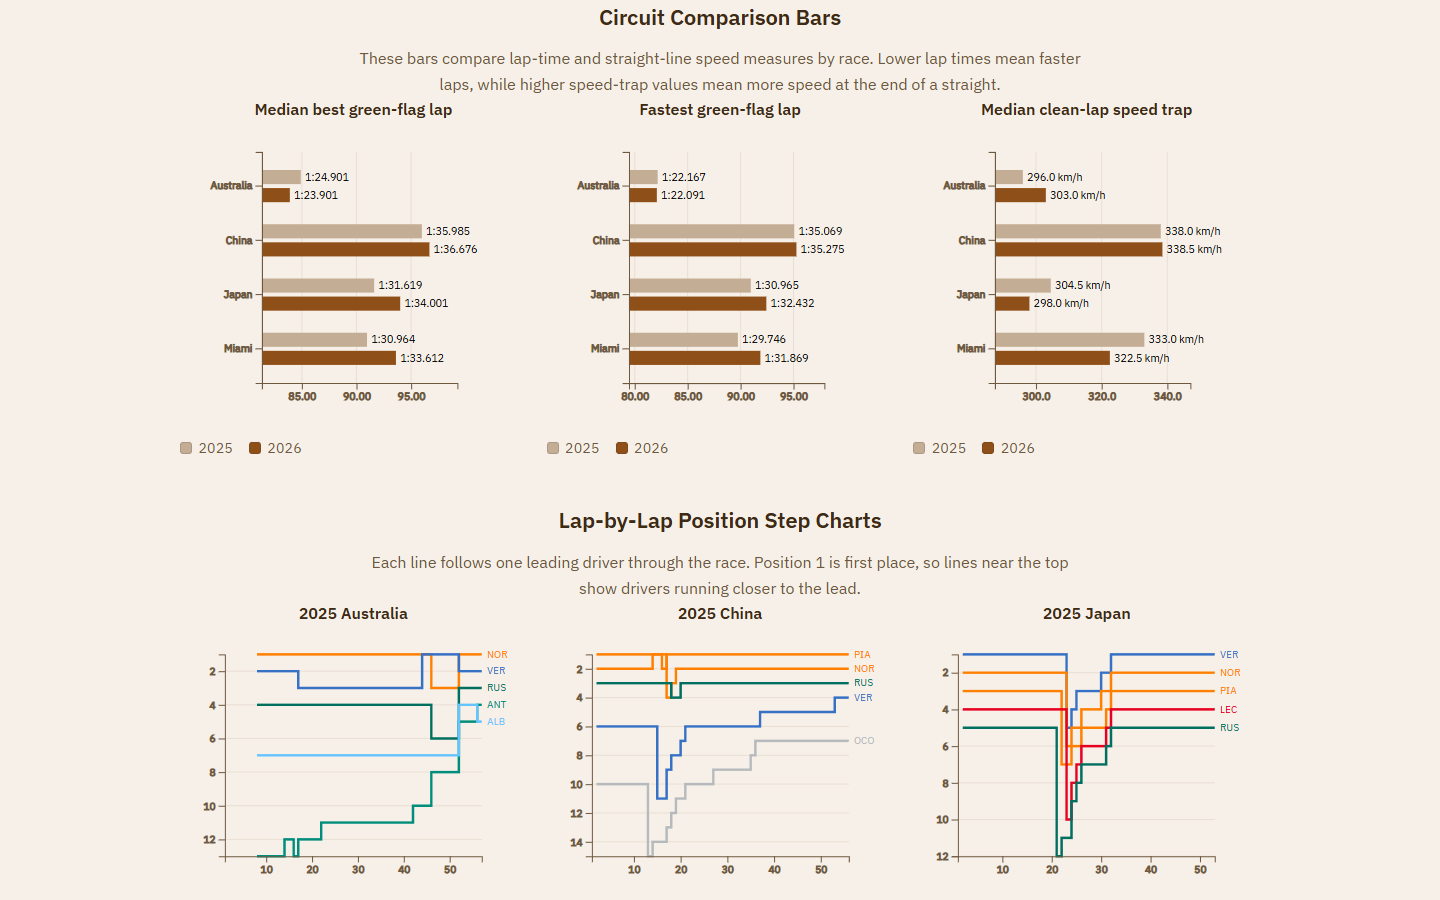
\includegraphics[width=\columnwidth]{figures/pace-bars.png}
    \caption{The pace section uses horizontal comparison bars for same-circuit metrics. Viewers should compare both direction and size of the 2025-to-2026 deltas, such as Australia becoming faster while Miami became slower in the available race data.}
    \label{fig:pace}
\end{figure}

\begin{figure}[t]
    \centering
    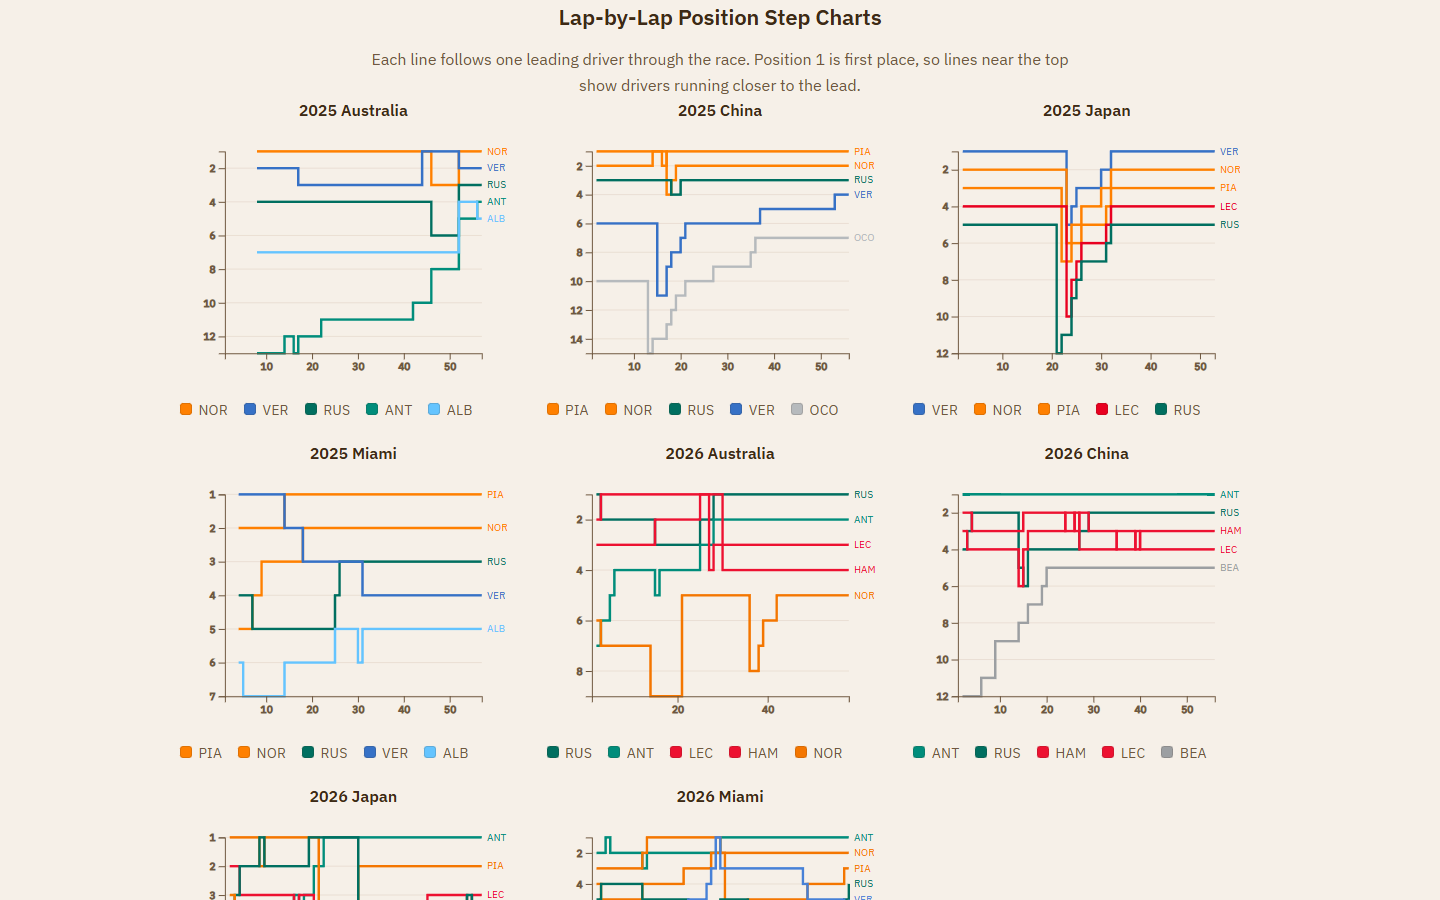
\includegraphics[width=\columnwidth]{figures/position-charts.png}
    \caption{The position section uses lap-by-lap step charts and a position-change proxy. Lines near the top represent drivers closer to first place, while the proxy summarizes how much the field order changed.}
    \label{fig:position}
\end{figure}

\subsection{Prototypes and Feedback}
The project went through several interface versions. The early site was functional but plain, as shown in Fig.~\ref{fig:early}. It later gained legends, tooltips, better numeric formatting, color improvements, chart descriptions, and the Miami 2025 and 2026 data. A more ambitious arcade/scrollytelling prototype was also attempted, shown in Fig.~\ref{fig:arcade}. That version had more personality and stronger transitions, but it added complexity quickly. The final site keeps fullscreen arcade transition moments and a stylized footer, but it does not depend on a fully animation-driven reading experience.

\begin{figure}[t]
    \centering
    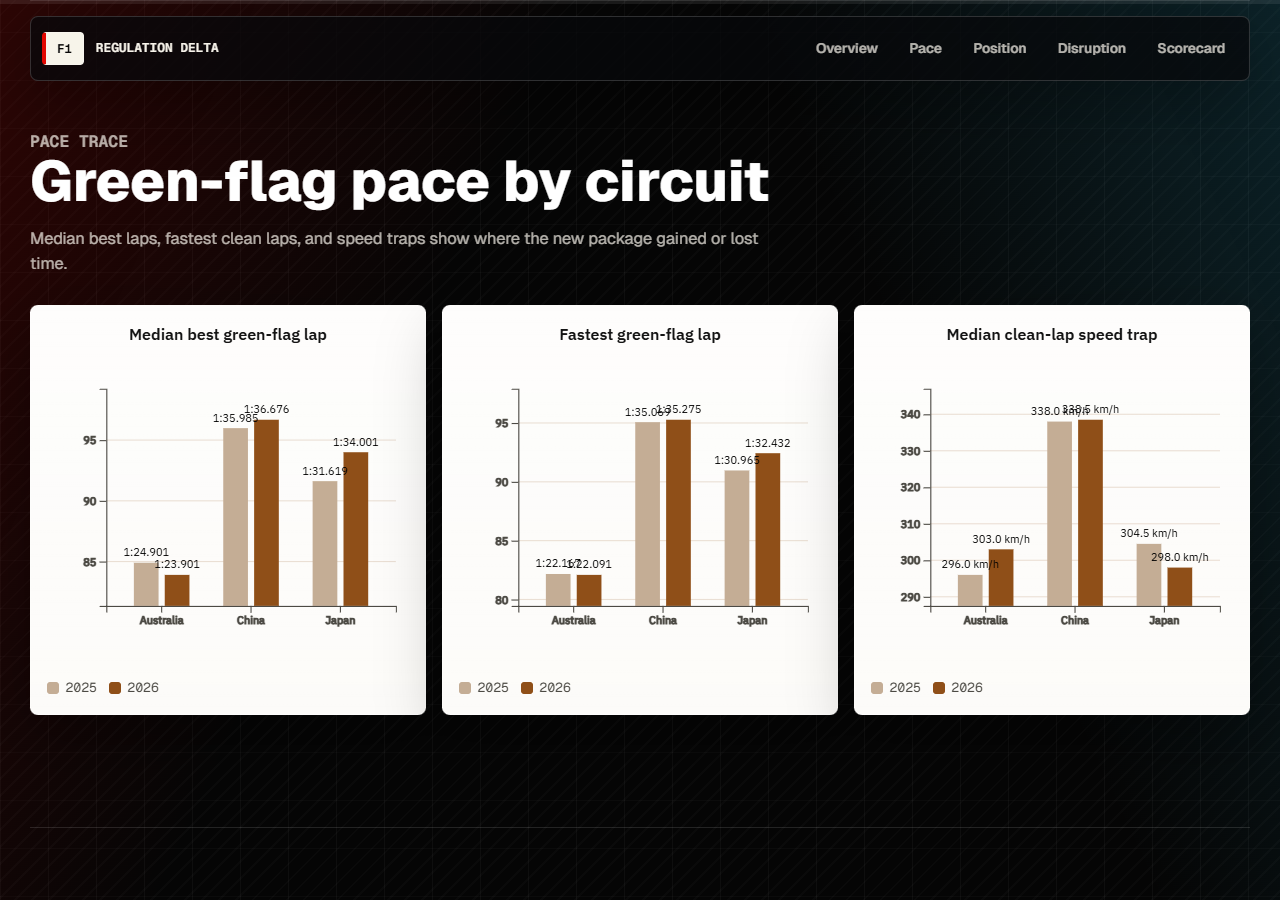
\includegraphics[width=\columnwidth]{figures/early-pace-prototype.png}
    \caption{An earlier prototype focused on getting the charts working before the final explanatory layer. It was less effective for non-F1 readers because it relied more heavily on labels and chart titles alone.}
    \label{fig:early}
\end{figure}

\begin{figure}[t]
    \centering
    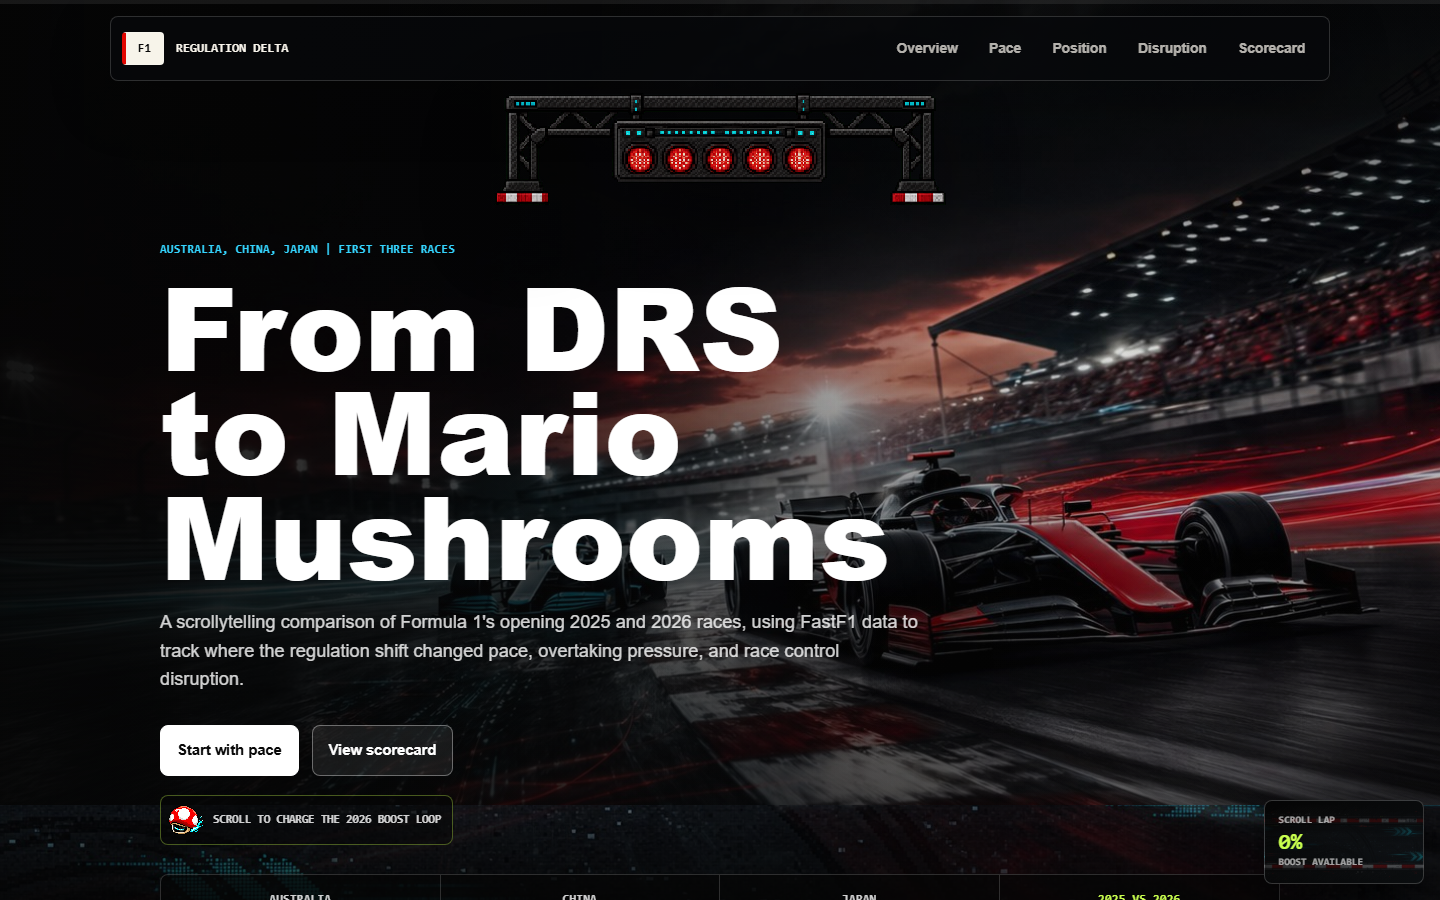
\includegraphics[width=\columnwidth]{figures/arcade-experiment.png}
    \caption{The arcade/scrollytelling experiment explored a stronger visual metaphor. The idea was promising, but a fully animated article introduced extra frontend complexity that was not worth the risk for the final class deliverable.}
    \label{fig:arcade}
\end{figure}

\subsection{Implementation Pieces}
Several pieces had to work together to execute the approach:
\begin{itemize}
    \item A FastF1 data script that can rebuild the race payloads and cache API data locally.
    \item A cleaned JSON/JavaScript data bundle that keeps the web page static and deployable through GitHub Pages.
    \item D3 renderers for bars, step charts, slope graphs, timelines, legends, scorecards, and tooltips.
    \item CSS for the retro visual theme, responsive chart layout, scrollytelling transitions, and footer.
    \item Manual and browser-based verification that the local page renders, the assets load, and the chart sections remain readable.
\end{itemize}

\subsection{Problems Encountered}
The most important data problem was interpreting FastF1 track-status values correctly. The first version made the incident timeline misleading by showing too many events as yellow flags. The fix was to separate yellow flags, VSC, Safety Car, and red flag status before aggregating them by lap.

The most important visual problem was balancing personality with readability. Formula 1 and Mario-inspired graphics made the project memorable, but too much motion or game-like decoration competed with the charts. The final version uses arcade transitions between sections while keeping the actual chart surfaces quieter.

The final problem was audience knowledge. Beta feedback made it clear that many viewers did not know what they were looking at. This led to short descriptions before each chart, legends, clearer tooltips, and less precise numeric formatting where additional decimals did not add useful meaning.

\section{Results}
The final page covers twelve circuits and both seasons. The data pipeline produced twenty-four race payloads. The main numeric outcomes are summarized in Table~\ref{tab:metrics}. Australia became faster in median best lap time by about 1.000 seconds, while the other eleven matched circuits were slower; Belgium showed the largest increase at 4.525 seconds. Caution-affected laps increased from 96 to 97 across the matched races, while fully neutralized laps decreased from 75 to 69. Monaco had the largest increase in fully neutralized laps, rising from 3 to 11.

\begin{table*}[t]
\caption{Selected Race Metrics Derived from FastF1}
\label{tab:metrics}
\centering
\begin{tabular}{lrrrrrr}
\hline
Race & Median Best Lap (s) & Fastest Lap (s) & Speed Trap (km/h) & Position Movement & Neutralized Laps & Not Classified \\
\hline
2025 Australia & 84.901 & 82.167 & 296.0 & 178 & 20 & 6 \\
2025 China & 95.985 & 95.069 & 338.0 & 342 & 0 & 4 \\
2025 Japan & 91.619 & 90.965 & 304.5 & 246 & 0 & 0 \\
2025 Miami & 90.964 & 89.746 & 333.0 & 161 & 6 & 4 \\
2025 Canada & 74.947 & 74.119 & 336.5 & 402 & 4 & 2 \\
2025 Monaco & 74.866 & 73.221 & 284.0 & 176 & 3 & 2 \\
2025 Barcelona & 77.998 & 75.743 & 338.0 & 417 & 6 & 2 \\
2025 Austria & 69.550 & 67.924 & 315.0 & 341 & 3 & 4 \\
2025 Great Britain & 90.818 & 89.337 & 323.0 & 402 & 14 & 5 \\
2025 Belgium & 106.550 & 104.861 & 316.5 & 230 & 4 & 0 \\
2025 Hungary & 80.581 & 79.409 & 309.5 & 355 & 0 & 1 \\
2025 Netherlands & 73.815 & 72.271 & 323.0 & 307 & 15 & 2 \\
2026 Australia & 83.901 & 82.091 & 303.0 & 190 & 7 & 6 \\
2026 China & 96.676 & 95.275 & 338.5 & 275 & 4 & 7 \\
2026 Japan & 94.001 & 92.432 & 298.0 & 215 & 6 & 2 \\
2026 Miami & 93.612 & 91.869 & 322.5 & 252 & 6 & 4 \\
2026 Canada & 75.845 & 74.210 & 332.0 & 241 & 5 & 6 \\
2026 Monaco & 76.332 & 73.481 & 280.0 & 133 & 11 & 6 \\
2026 Barcelona & 81.726 & 80.122 & 349.5 & 399 & 5 & 5 \\
2026 Austria & 71.587 & 70.374 & 319.0 & 325 & 4 & 4 \\
2026 Great Britain & 93.649 & 91.777 & 330.5 & 258 & 7 & 2 \\
2026 Belgium & 111.075 & 108.890 & 305.0 & 222 & 7 & 3 \\
2026 Hungary & 83.932 & 82.000 & 338.0 & 362 & 2 & 3 \\
2026 Netherlands & 76.134 & 74.230 & 321.0 & 423 & 5 & 5 \\
\hline
\end{tabular}
\end{table*}

\subsection{Objective Alignment}
Table~\ref{tab:objectivealignment} maps each visualization to the objective it supports. The design intentionally avoids making one chart answer every question. The first bars answer pace and speed questions, the lap charts answer position-flow questions, the timeline answers disruption questions, and the scorecard synthesizes the whole comparison.

\begin{table*}[t]
\caption{Visualization Alignment with Project Objectives}
\label{tab:objectivealignment}
\centering
\begin{tabular}{p{0.25\textwidth}p{0.18\textwidth}p{0.48\textwidth}}
\hline
Visualization & Objective(s) & What the viewer should observe \\
\hline
Circuit comparison bars & Objective 1 & Same-circuit differences in median best lap, fastest lap, and speed-trap values between 2025 and 2026. \\
Lap-by-lap position charts & Objective 2 & How the leading drivers moved through the race, including stable leaders, pit-cycle changes, and late-race movement. \\
Position-change slope graph & Objective 2 & Whether the running order became more or less volatile at each circuit from 2025 to 2026. \\
Incident and neutralization timeline & Objective 3 & Where caution periods, Safety Cars, VSCs, red flags, and normal green-flag laps occurred. \\
Final circuit scorecard & Objectives 1--4 & A compact comparison of every metric and circuit so the viewer can see cross-circuit patterns without reading each chart again. \\
\hline
\end{tabular}
\end{table*}

\begin{figure}[t]
    \centering
    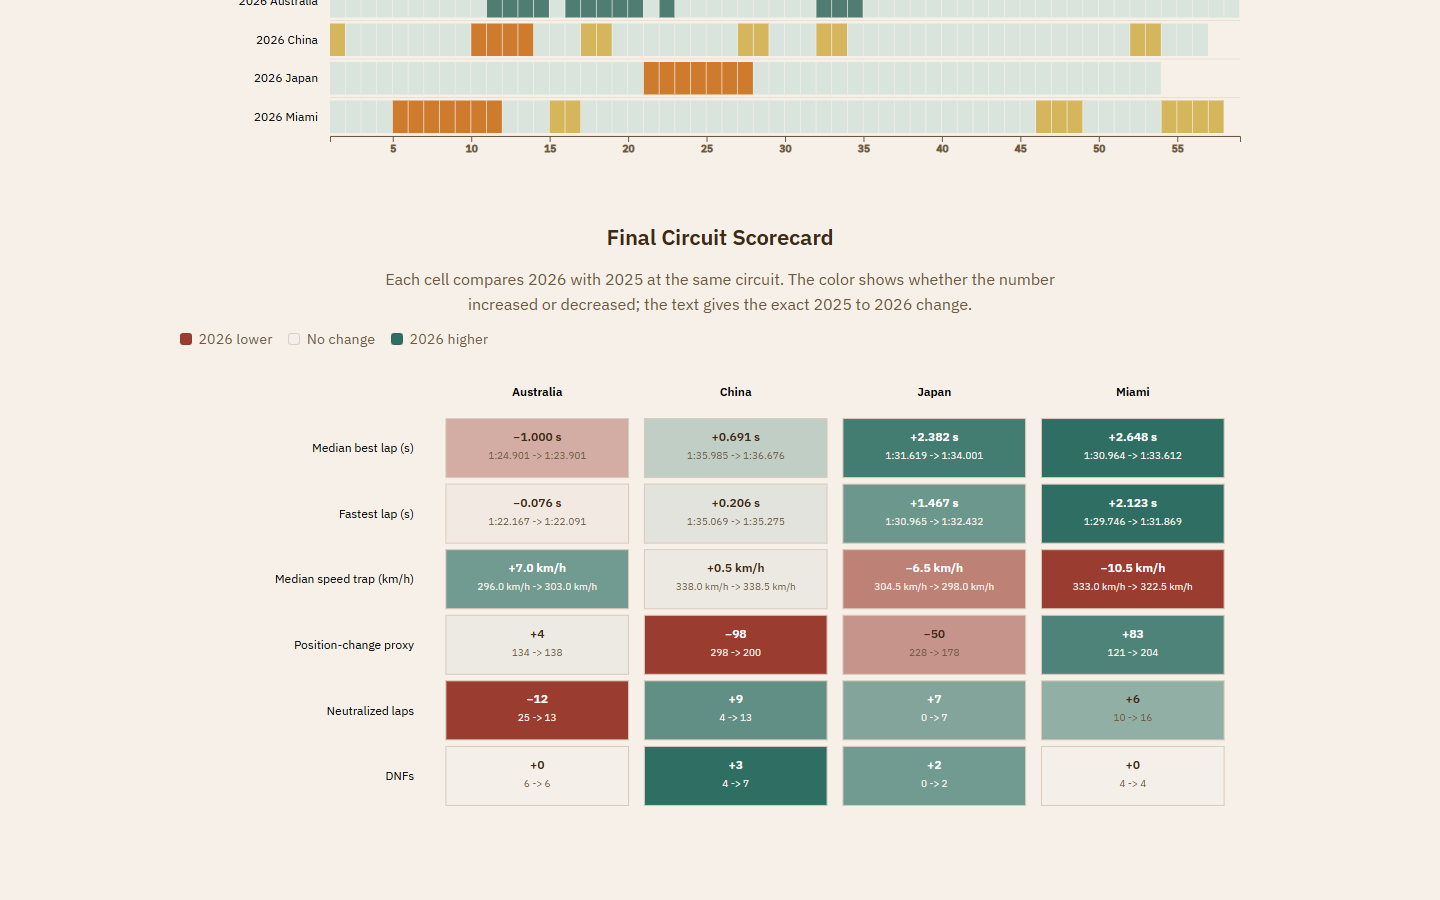
\includegraphics[width=\columnwidth]{figures/scorecard.png}
    \caption{The scorecard summarizes the full project by showing the 2026 minus 2025 delta for each circuit and metric. The color legend helps the viewer see which metrics increased or decreased before reading exact values.}
    \label{fig:scorecard}
\end{figure}

\subsection{Measuring Success}
Success was measured by objective completion rather than by a single performance metric. The final site succeeds if it:
\begin{enumerate}
    \item Covers every planned race after adding the latest completed 2025 and 2026 race pair.
    \item Provides a visualization for each major objective.
    \item Makes the charts understandable to viewers who do not already follow Formula 1.
    \item Incorporates beta feedback into concrete changes.
    \item Remains stable enough for a live class presentation and GitHub Pages deployment.
\end{enumerate}

On these criteria, the project is successful as a final class deliverable. It is not yet a rigorous motorsport analytics study, and it does not claim causality between 2026 regulations and every observed difference. Its success is instead that it gives viewers a structured way to explore the comparison.

\section{Discussion}
The approach is promising because it breaks a complex racing question into smaller, explainable comparisons. Same-circuit comparisons help avoid some of the noise of comparing unrelated tracks. Multiple chart types also prevent a single metric, such as final finishing order, from dominating the story. The scorecard is especially useful because it makes the final conclusion cautious: some metrics moved in opposite directions depending on the circuit.

A better variant would be a fuller scrollytelling article where the reader moves from lights out to the checkered flag and the same visual elements evolve across the page. Scrollama could support this by connecting scroll position to section state, chart highlights, and vehicle animations \cite{scrollama}. However, this should be done only after the chart pipeline and data validation are stable. The project showed that motion can improve engagement, but it can also distract from the data if it is added before the analytical structure is clear.

The main lesson was that approachable visualization requires explanation at several levels. A chart title is not enough when the audience may not know what a Safety Car or speed trap means. Short chart descriptions, legends, and good tooltips are not decoration; they are part of the visualization design. Another lesson was that data cleaning and semantic interpretation matter as much as chart rendering. The safety-car bug changed the meaning of an entire chart until the status codes were interpreted more carefully.

If starting again, I would collect visual references earlier and write down the visual language before polishing individual charts. I would also build validation checks sooner, especially for incident states, missing laps, and unexpected FastF1 fields. Finally, I would prototype animations separately from the main site before integrating them into the deliverable.

\section{Future Work}
With more time, I would add:
\begin{itemize}
    \item A stronger scrollytelling mode where charts animate from section to section.
    \item More Formula 1 and retro-game references, such as pit-stop powerups or Mario Kart-style transition scenes, while keeping chart surfaces readable.
    \item Driver and team filters for deeper exploration.
    \item Lap replay controls for the position charts and incident timeline.
    \item More seasons, more circuits, qualifying data, sprint race context, tire strategy, and weather summaries.
    \item More robust validation around FastF1 fields and race-control status codes.
    \item Accessibility checks for color contrast, reduced motion, keyboard navigation, and tooltip alternatives.
\end{itemize}

\section{Conclusion}
\emph{From DRS to Mario Mushrooms} demonstrates that Formula 1 race data can be made more understandable through a guided set of targeted visualizations. The final site compares early 2025 and 2026 races across pace, speed, position movement, neutralization, and circuit-level summaries. The project also shows the tradeoff between visual personality and analytical clarity: arcade styling helped make the project memorable, but the charts needed concise explanations and restrained interaction to stay readable. The result is a practical final project that can support a live demo, a presentation, and further development into a richer scrollytelling article.

\bibliographystyle{IEEEtran}
\bibliography{references}

\end{document}
